\documentclass[11pt]{hmcpset}
\usepackage[margin=1in]{geometry}
\usepackage{amsmath,amssymb,enumerate,graphicx,url}

\newcommand{\ket}[1]{|#1\rangle}
\newcommand{\bra}[1]{\langle #1|}
\newcommand{\braket}[2]{\langle #1|#2\rangle}
\newcommand{\braketop}[3]{\langle #1| #2 | #3 \rangle}
\newcommand{\normsq}[1]{\left|#1\right|^2}
\newcommand{\prob}[2]{\normsq{\braket{#1}{#2}}}
\newcommand{\avg}[1]{\langle #1 \rangle}


\usepackage{xcolor}
\usepackage{listings}

\definecolor{mGreen}{rgb}{0,0.6,0}
\definecolor{mGray}{rgb}{0.5,0.5,0.5}
\definecolor{mPurple}{rgb}{0.58,0,0.82}
\definecolor{backgroundColour}{rgb}{0.95,0.95,0.92}

\lstdefinestyle{Python}
{
	language=Python,
	backgroundcolor=\color{backgroundColour},   
	commentstyle=\color{mGreen},
	keywordstyle=\color{magenta},
	numberstyle=\tiny\color{mGray},
	stringstyle=\color{mPurple},
	basicstyle=\footnotesize\ttfamily,
	breakatwhitespace=false,         
	breaklines=true,                 
	captionpos=b,                    
	keepspaces=true,                 
	%numbers=left,                    
	numbersep=5pt,                  
	showspaces=false,                
	showstringspaces=false,
	showtabs=false,                  
	tabsize=3
}



\name{}
\class{PHYS134}
\assignment{Section on Gaussian Beams}
\duedate{2021-02-22}

\begin{document}
%\problemlist{Steck: }



%===========================================================
\begin{problem}[Steck 6.13 (5\,pts)]
	Consider two monochromatic, Gaussian beams: a ``red'' beam of frequency $\omega$, and a ``blue'' beam
	of frequency $2\omega$. Both have identical transverse intensity profiles at their respective foci, which both occur at the origin. Describe completely how the geometries (both near- and far-field) of the two fields differ. 
	
	\textit{Jason's Note:} Draw a picture of the two overlapping beams (like the figure on page 94) in two different colors. Try to be somewhat accurate about what might be 2$\times$ or 4$\times$ as big: the far-field diverge angles, the depth-of-focus parameters $z_0$ for each beam. You could even make a proper plot in python or Mathematica.
\end{problem}

\begin{solution}
	\vfill
\end{solution}
\pagebreak



%===========================================================
\begin{problem}[Steck 6.1 (5\,pts)]
	A common technique in the laboratory for measuring the beam waist parameter of a Gaussian beam 	is illustrated in the diagram. A Gaussian beam is incident on an optical power meter, which registers 	the total power of the incident beam. A knife edge can be translated in the transverse direction to 	block part of the beam (i.e., if the position of the knife edge is $x_\mathrm{knife}$, then the parts of the beam with $x < x_\mathrm{knife}$ is blocked from reaching the power meter). The ``10-90'' rule is to measure the knife edge position $x_{10\%}$ where the power meter reads 10\% of the total beam power, and then the position	$x_{90\%}$ where the power meter reads 90\% of the total beam power. Then the beam radius $w(z)$ at the knife-edge location z along the beam is given by
	\[
	w(z) = \alpha \left| x_{10\%} - x_{90\%} \right|,
	\]
	where $\alpha$ is some constant factor. Calculate the numerical value of $\alpha$.
	
	\begin{center}
		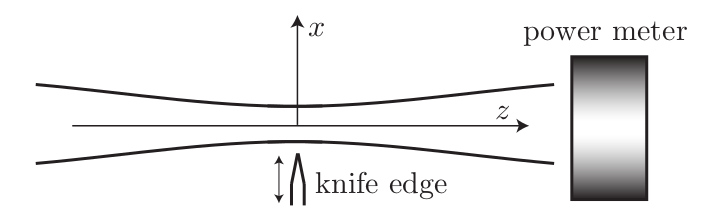
\includegraphics[width=0.49\textwidth]{knife_edge_beam}
	\end{center}

\textit{Jason's Note:} The figure above shows this setup for the special case where the waist $w_0$ is measured. Be sure to justify why this works at any $z$ position to get $w(z)$.

\textit{Another Note:}	Below is is what things look like right at the knife edge. Some people asked about diffraction after the knife edge. Yes, this will happen, and we will calculate it later, but all of that light is going to go into a single power meter measurement, so it doesn't matter.

\begin{center}
	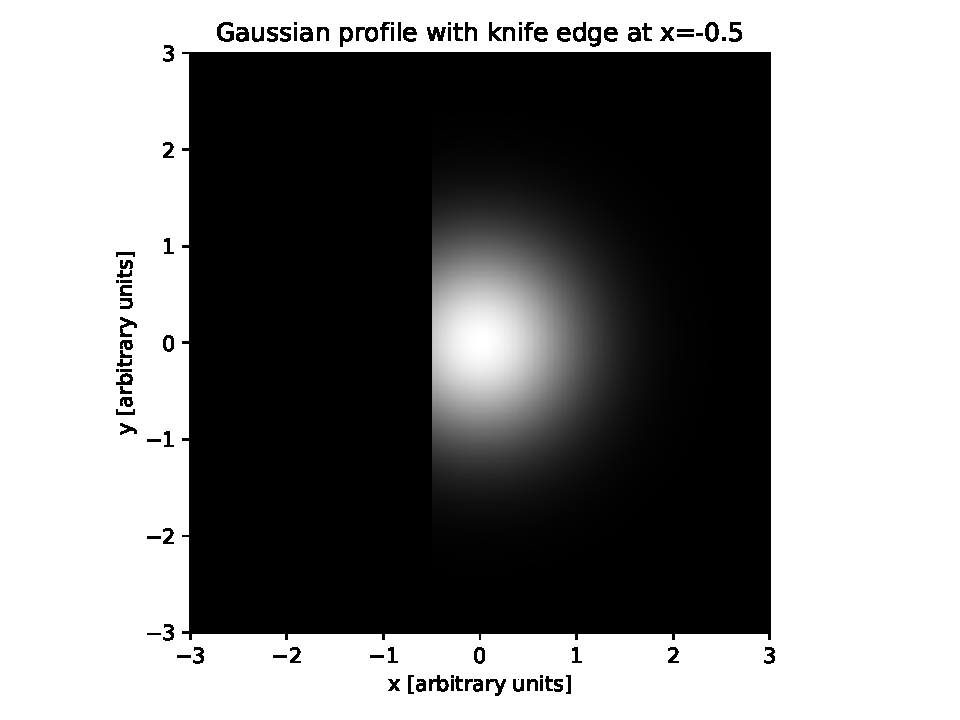
\includegraphics[width=0.49\textwidth]{knife_edge_gaussian}
\end{center}

	\textit{Still More Notes:} The integrals are no longer cylindrically symmetric and they don't go from $-\infty$ to $\infty$. Mathematica can really help here, since there's no closed-form solution. If you don't want to Mathematicate, you'll need to get your solution into the form of the so-called Error function and look up values numerically: \url{https://en.wikipedia.org/wiki/Error_function}
	
	Pyhon can compute the error function and its inverse numerically:
	\begin{lstlisting}[style=Python]
import scipy.special
scipy.special.erf(1) # error function, example evaluating it at 1
scipy.special.erfinv(0.843) # example inverse error function 
	\end{lstlisting}
\end{problem}
%\begin{solution}
%	\vfill
%\end{solution}
\pagebreak






%===========================================================
\begin{problem}[Steck 6.7 (5\,pts)]
	Verify that the compact form for the Gaussian beam in terms of the complex beam parameter,
	Eq. (6.41),
	\[
	E^{(+)}(\mathbf{r}) = E^{(+)}_0 \frac{q_0}{q(z)}
	\exp \left[ \frac{i k r^2}{2q(z)} \right] 
	\exp(ikz)
	\]
	is equivalent to the standard form for the Gaussian beam, Eq. (6.10),
	\[
	E^{(+)}(\mathbf{r}) = E^{(+)}_0 \frac{w_0}{w(z)}
	\exp \left[ - \frac{r^2}{w^2(z)} \right] 
	\exp \left[ikz - i \tan^{-1}\left(\frac{z}{z_0}\right) \right] 
	\exp \left[ i k \frac{r^2}{2R(z)} \right] 
	\]
	
	\textit{Note 1}: $q=z-i z0$. Also, the first equation here is correct without the square root. The actual 6.14 on page 98 has no square root. The square root in the book's problem statement is wrong.
	
	\textit{Note 2}: To deal with the square root of a complex number, write it in the magnitude-phase form of $\rho e^{i\theta}$. I'm 95\% sure the square root is right, but check the arctangent and let me know.
\end{problem}

\begin{solution}
	\vfill
\end{solution}
\pagebreak



\end{document}
